% repo/sica-plugin/docs/paper/main.tex
%
% Setdrift MSR-targeted methodology paper — acmart (sigconf) skeleton.
%
% D8-07: this is a REAL paper skeleton with the actual section headings the
% Phase 10 (DELIV-04) methodology paper draft will fill in — not a throwaway
% 1-page compile test. D8-09: venue template is acmart sigconf (ACM-family
% stand-in for MSR's own format; swap at Phase 10 submission time if needed).
%
% Compile sequence (bibtex, NOT biber — see README.md):
%   pdflatex main.tex && bibtex main && pdflatex main.tex && pdflatex main.tex
%
\documentclass[sigconf]{acmart}

\begin{document}

\title{Setdrift: Configuration Drift Detection and Repair for AI Coding-Agent Configuration}

\author{Trung Nguyen}
\affiliation{%
  \institution{FSB — MSE Capstone}
  \country{Vietnam}
}

\begin{abstract}
[PLACEHOLDER — Phase 10 (DELIV-04) fills in the real abstract once
evidence-run results land. Source paragraph for the Setdrift/Robeyns
name-collision differentiator: see
\texttt{.planning/codebase/dissertation-abstract-name-note.md} — reuse that
145-word paragraph verbatim as the starting point, then extend with the
real survive/null/die outcome once Phase 7 evidence lands.]
\end{abstract}

\maketitle

\section{Introduction}
[PLACEHOLDER — Phase 10 (DELIV-04). Frames the falsifiable claim (design doc
\S1, \texttt{repo/sica-plugin/docs/design/2026-05-20-falsifiable-claim.md})
and the observe→diagnose→patch→verify loop as the paper's contribution.]

\section{Related Work}
Setdrift shares its name with, but targets a fundamentally different layer of
the system than, Robeyns et al.'s Self-Improving Coding Agent
\cite{robeyns2025selfimproving}, which edits an agent's own source code to
improve its own implementation. Setdrift instead optimizes AI-coding-agent
\emph{configuration} — skills, hooks, sub-agents, MCP wiring, CLAUDE.md — and
treats source-code self-modification as an explicit anti-goal. [PLACEHOLDER —
Phase 10 (DELIV-04) extends this section with the full five-axis
differential (Chapter 2 of the dissertation) and the competitor-differential
one-pager (WRITE-01).]

\section{Methodology}
[PLACEHOLDER — Phase 10 (DELIV-04). Skill-trigger macro-F1 as the primary
metric, the three experiment arms (A/B/C), and the GEPA-based optimizer loop.]

\section{Corpus Construction}
[PLACEHOLDER — Phase 10 (DELIV-04). GitBug-Java-derived public corpus, the
heuristic-mining precision gate, and inter-rater agreement methodology.]

\section{Results}
[PLACEHOLDER — GATED ON REAL F1 (Phase 7 evidence runs, RUN-01..06). Phase 10
(DELIV-04) mechanically selects the matching survive/null/die branch template
from \texttt{.planning/dissertation/06-results-\{survive,null,die\}.md} once
real numbers land — this section cannot be drafted before that gate opens.]

\begin{figure}[h]
  \centering
  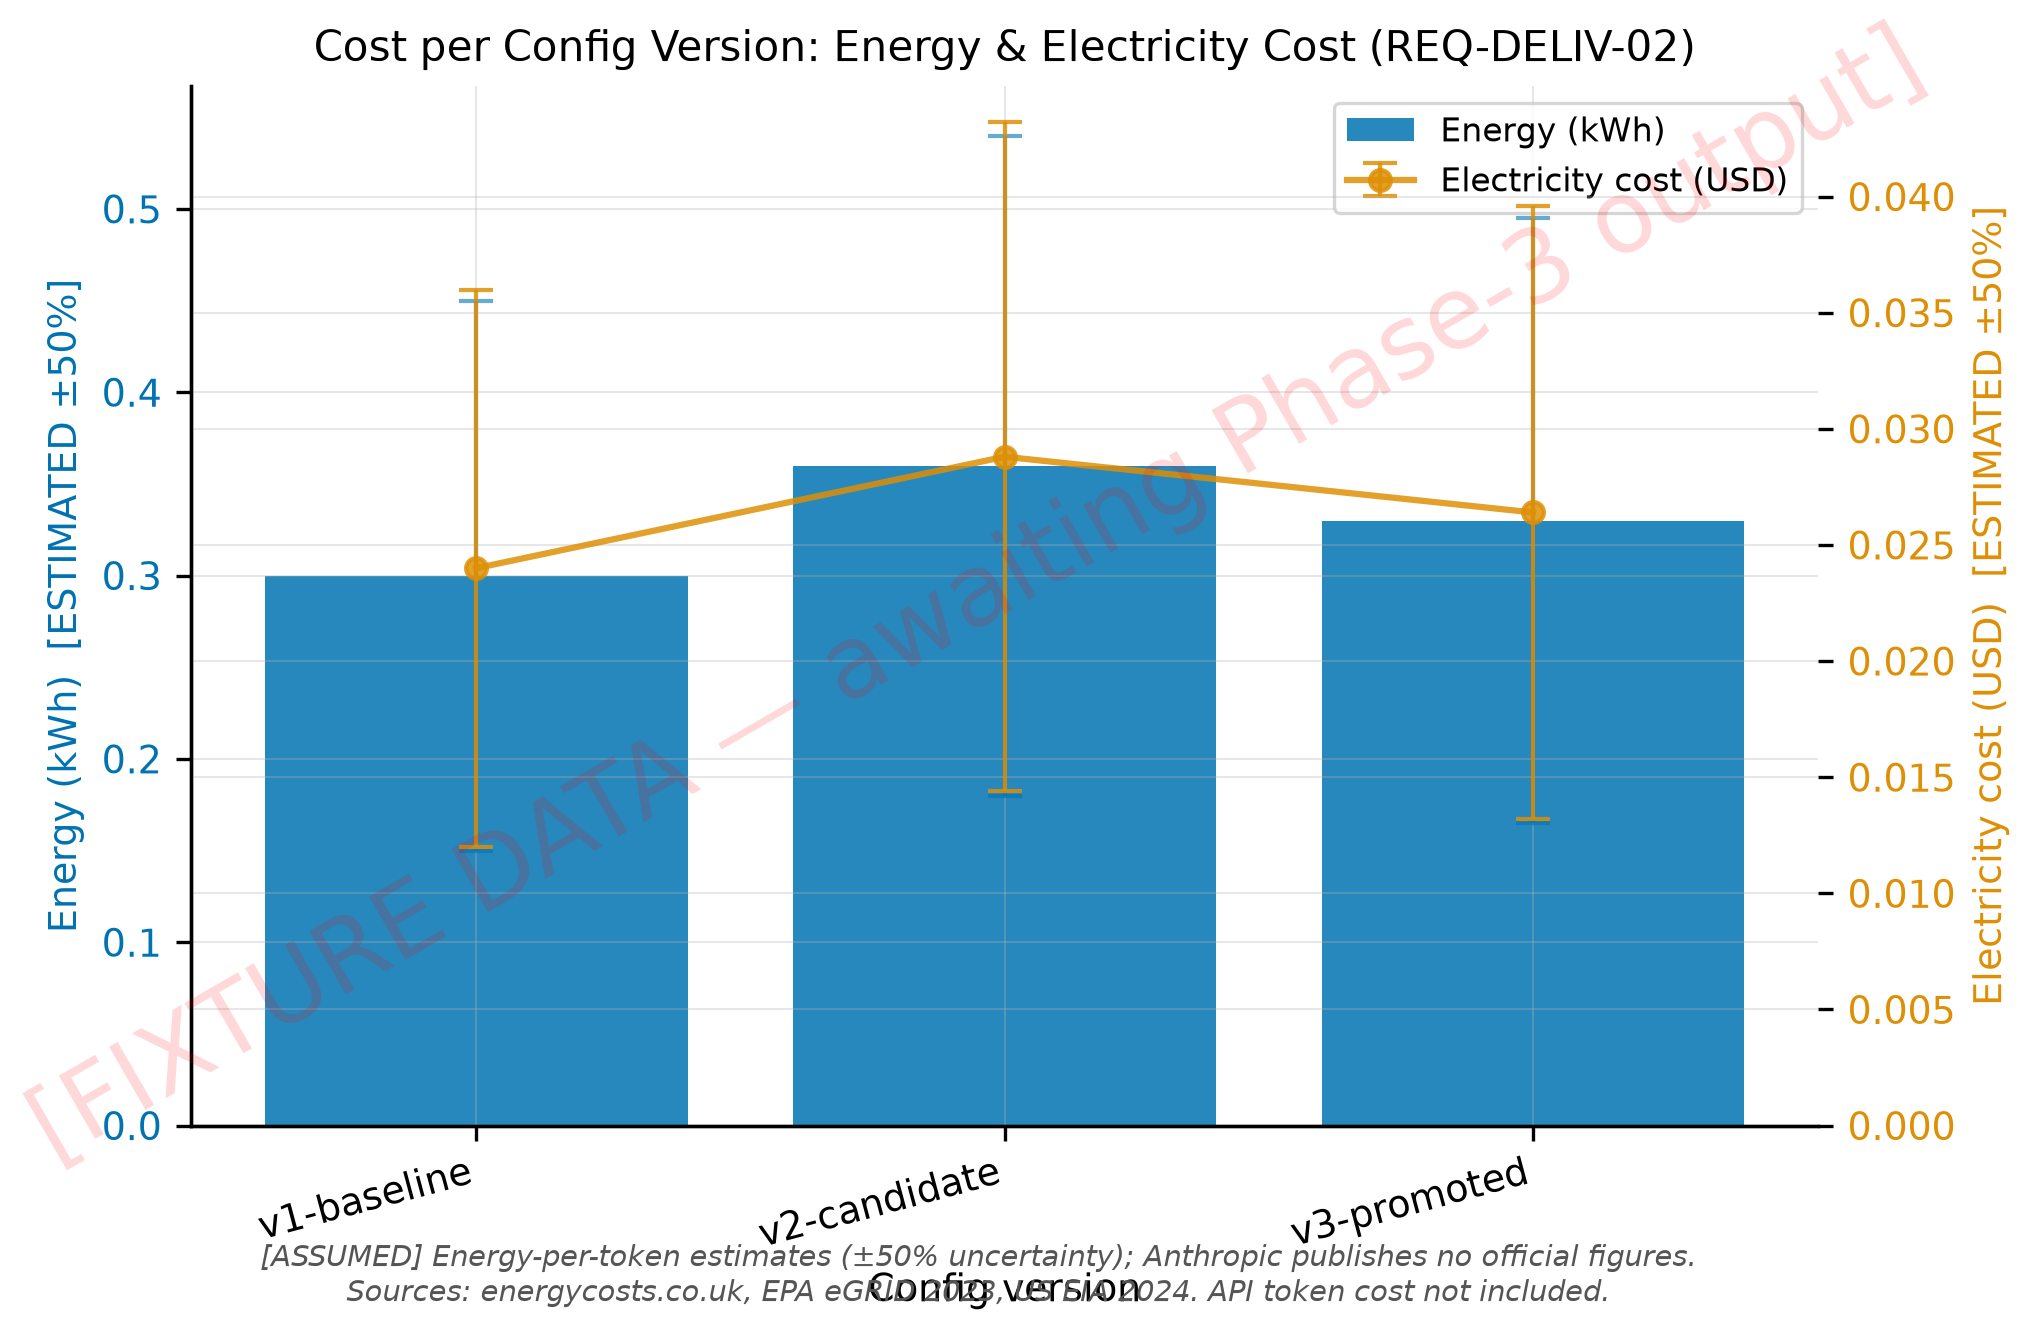
\includegraphics[width=0.8\linewidth]{figures/cost-delta.png}
  \caption{FIXTURE DATA — this figure is watermarked synthetic data used
  solely to verify the acmart \texttt{\textbackslash includegraphics} +
  compile pipeline (WRITE-02 compile-smoke-test only, D-09). It is not
  dissertation content and will be replaced by Phase 9 (FIG-01) with a real,
  unwatermarked cost-delta figure once real experiment data lands.}
  \label{fig:cost-delta-fixture}
\end{figure}

\section{Threats to Validity}
[PLACEHOLDER — Phase 10 (DELIV-04). See
\texttt{.planning/dissertation/07-threats-to-validity.md} for the full-prose
threats-to-validity chapter drafted in this phase (WRITE-03); this section
is a compressed paper-length summary of that chapter.]

\section{Conclusion}
[PLACEHOLDER — Phase 10 (DELIV-04). Gated on the same survive/null/die
decision rule (design doc \S6) as the Results section.]

\bibliographystyle{ACM-Reference-Format}
\bibliography{references}

\end{document}
